%=============================================================================
% Thesis Template in LaTex
%
% File:  05-Resultate.tex -- Resultate
% Author(s): Cyrano Golliez <golliezc@student.ethz.ch>
%
% Creation:  27 Jan 2014
% Time-stamp: <Tue 2013-08-13 20:14 juergen>
%
% Copyright (c) 2014 Infrastructure Management Group (IMG)
%               http://ibi.ethz.ch
%
% More information on LaTeX: http://www.latex-project.org/
%=============================================================================

\chapter{Resultate}
\label{chap:Resultate}

Um die Verkehrssituation am Bahnübergang Brunnenstrasse nachhaltig zu verbessern, bedarfs es einer optimalen Variante, die durch den Vergleich der gemäss Abschnitt > berechneten Risiken der Varianten bestimmt wird. Der Vergleich der Risiken der Varianten erfolgt für die in Abschnitt < definierten Zustände um die gefunden optimale Lösung zu bestärken oder allenfalls zu verwerfen.
Nachfolgend dargestellt sind die Resulatet der Risikoberechnung sowie der Risikovergleich und die für die verschiedenen Zustände bestimmte optimale Variante. 

\begin{figure}[h!]
  \centering
  \subfloat[][]{\label{img:RisikoVar-Z0)}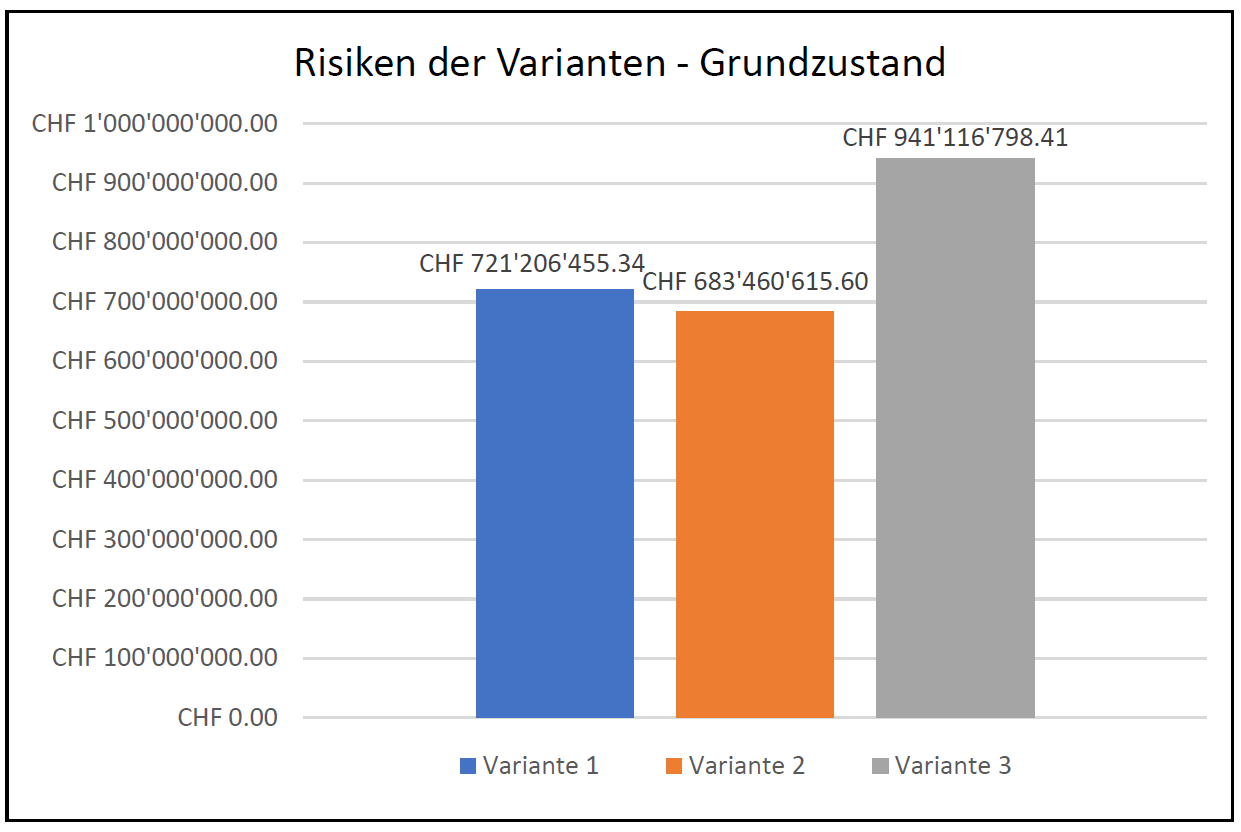
\includegraphics[width=.45\textwidth]{./figures/f-05-02-RisikenVarianteZ0}}
  \hfill
  \subfloat[][]{\label{img:VariantenwahlZ0)}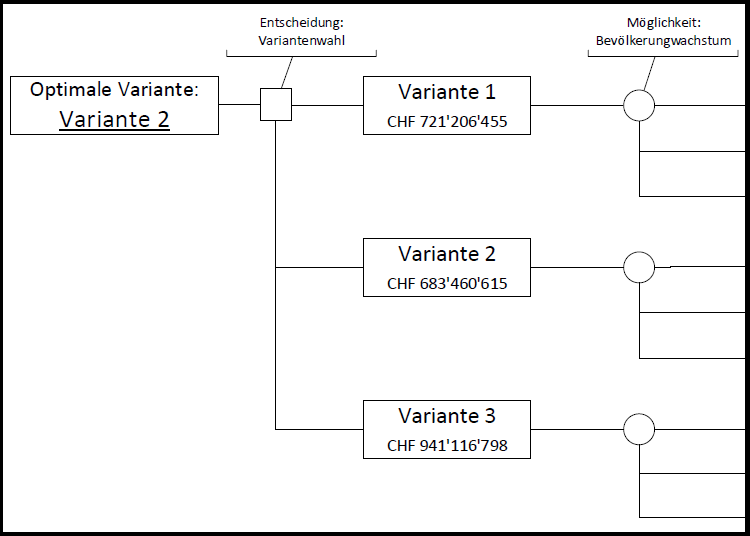
\includegraphics[width=.45\textwidth]{./figures/f-05-01-Variantenwahl}}
\caption[Verkehrsaufkommen]{Risikovergleich und Entscheidungsprozess im Zustand 0}
  \label{fig:Z4}
\end{figure}

\paragraph{Zustand 0}

Wie in der Abbildung \ref{img:RisikovergleichVarianten} ersichtlich, beträgt das Risiko der Variante 1 im Zustand 0 721'206'455 CHF, das Risiko der Variante 2 683'460'615 CHF und das Risiko der Variante 3 941'116'798 CHF. Das Risiko der Variante 2 ist somit um 37'745'840 CHF geringer als das Risiko der Variante 1 und um 257'656'183 CHF kleiner als das Risiko der Variante 3. Die Differenz der Risiken der Varianten 1 und 3 beträgt 219'910'343 CHF. \\
Die Variante mit dem geringsten Risiko im Zustand 0 ist demnach Variante 2 und ist dementsprechen die optimale Variante, wie in Abbildung \ref{img:VariantenwahlZ0} dargestellt.

\paragraph{Zustand 1 bis 3}

Die nachfolgende Abbildung stellt die Risiken der Varianten in den Zuständen 1 bis 3 dar. Es ist klar ersichtlich, dass sich in den Zuständen 1 bis 3 keine Veränderung der optimalen Lösung ergibt und weiterhin die Variante 2 die optimale Lösung darstellt. Aus diesem Grund verzichte ich auf die ausführliche Darstellung der Zustände 1 bis 3 und verweise auf den Abschnitt \ref{chap:Diskussion} in dem ich die Zustände vergleiche und diskutiere.

\begin{figure}[h!]
	\centering
	\includegraphics[width=\textwidth]{figures/f-05-00-01-RisikenVergleichZustände1-3}
	\caption[Risikovergleich der Zustände 1 bis 4]{Risiken der Varianten - Vergleich der Zustände 1 bis 3}
	\label{img:RisikovergleichVarianten}
\end{figure}

\paragraph{Zustand 4}

Im Zustand 4 beträgt das Risiko der Variante 1 wie im Zustand 0 721'206'455 CHF. Das Risiko der Variante 2 beträgt 683'460'616 CHF und das Risiko der Variante 3 ist mit 683'422'520 CHF deutlich niedriger als in Zustand 0. In Abbildung \ref{img:Z4-V2/V3)} wird der Vergleich der Varianten 2 und 3 gezeigt, wo man erkennen kann, dass die Differenz der berechneten Risiken 38'095 CHF beträgt.

Aufgrund der berechneten Risiken im Zustand 4 und unter den getroffenen Annahmen, ist die Variante 3 die optimale Lösung zur bedarfsgerechten Verbesserung der Verkehrssituation am Bahnübergang. Eine Diskussion dieser Lösung folgt im Abschnitt \ref{chap:Diskussion}.

\begin{figure}[h!]
  \centering
  \subfloat[][]{\label{img:RisikenZ4)}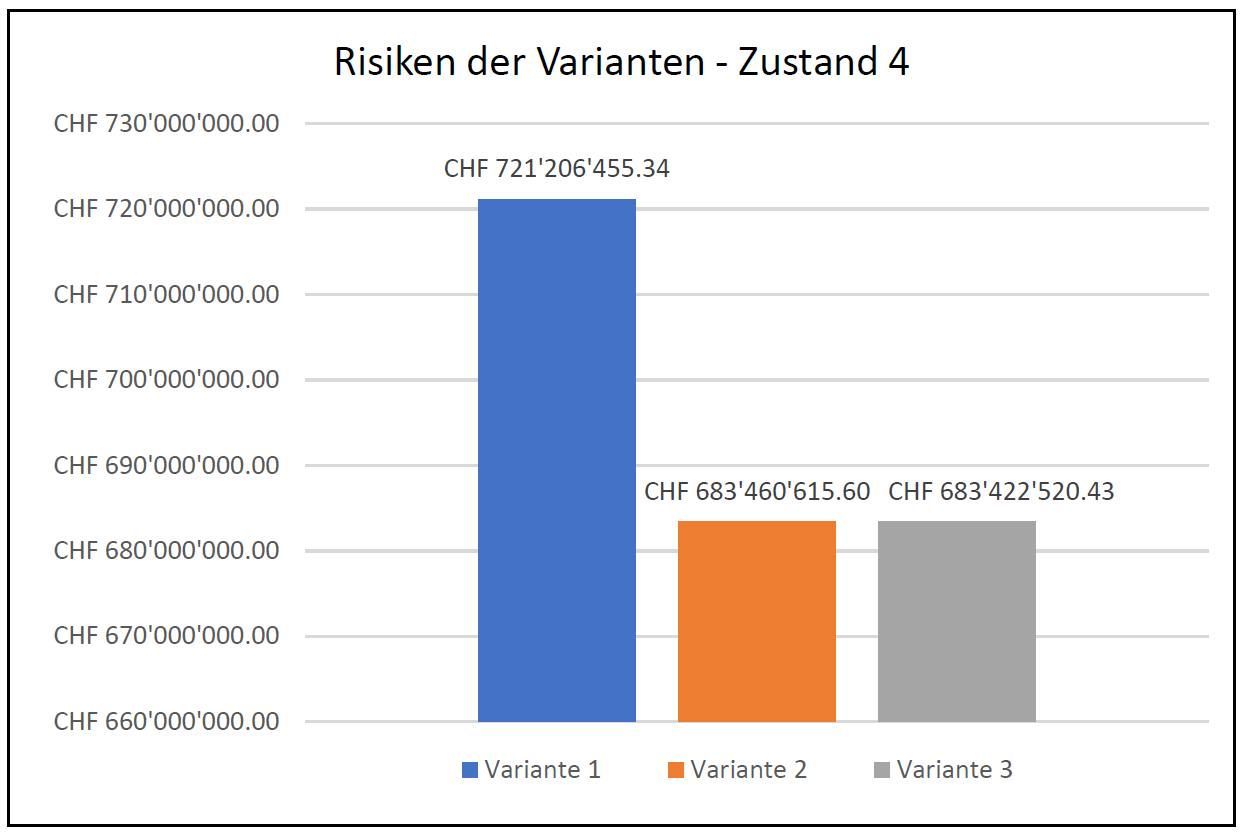
\includegraphics[width=.45\textwidth]{./figures/f-05-05-RisikenVarianteZ4}}
  \hfill
  \subfloat[][]{\label{img:Z4-V2/V3)}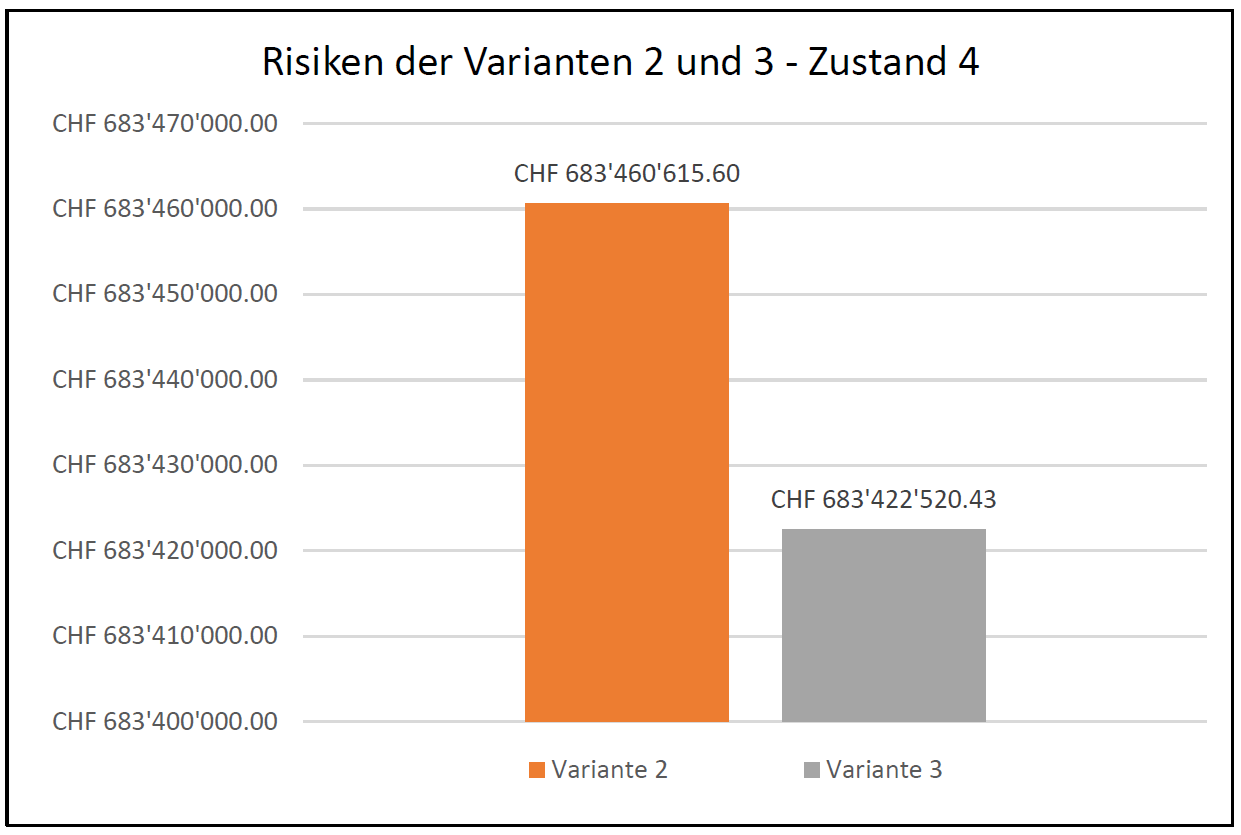
\includegraphics[width=.45\textwidth]{./figures/f-05-06-RisikenVariante-2und3-Z4}}
\caption[Verkehrsaufkommen]{Tägliches Verkehraufkommen Brunnenstrasse}
  \label{fig:Z4}
\end{figure}



% ===========================================================================
% EOF
%

%%% Local Variables:
%%% mode: latex
%%% TeX-master: "../main"
%%% End:
